\part*{Annexes}
\appendix
\renewcommand{\chaptermark}[1]{\markboth{\appendixname\ \thechapter: #1}{}}
\addcontentsline{toc}{part}{Annexes} %\mtcaddchapter

\chapter{Système de stabilisation en fréquence et de distribution des faisceaux laser}\label{app:laserlock}

\begin{figure}[h]
\centering
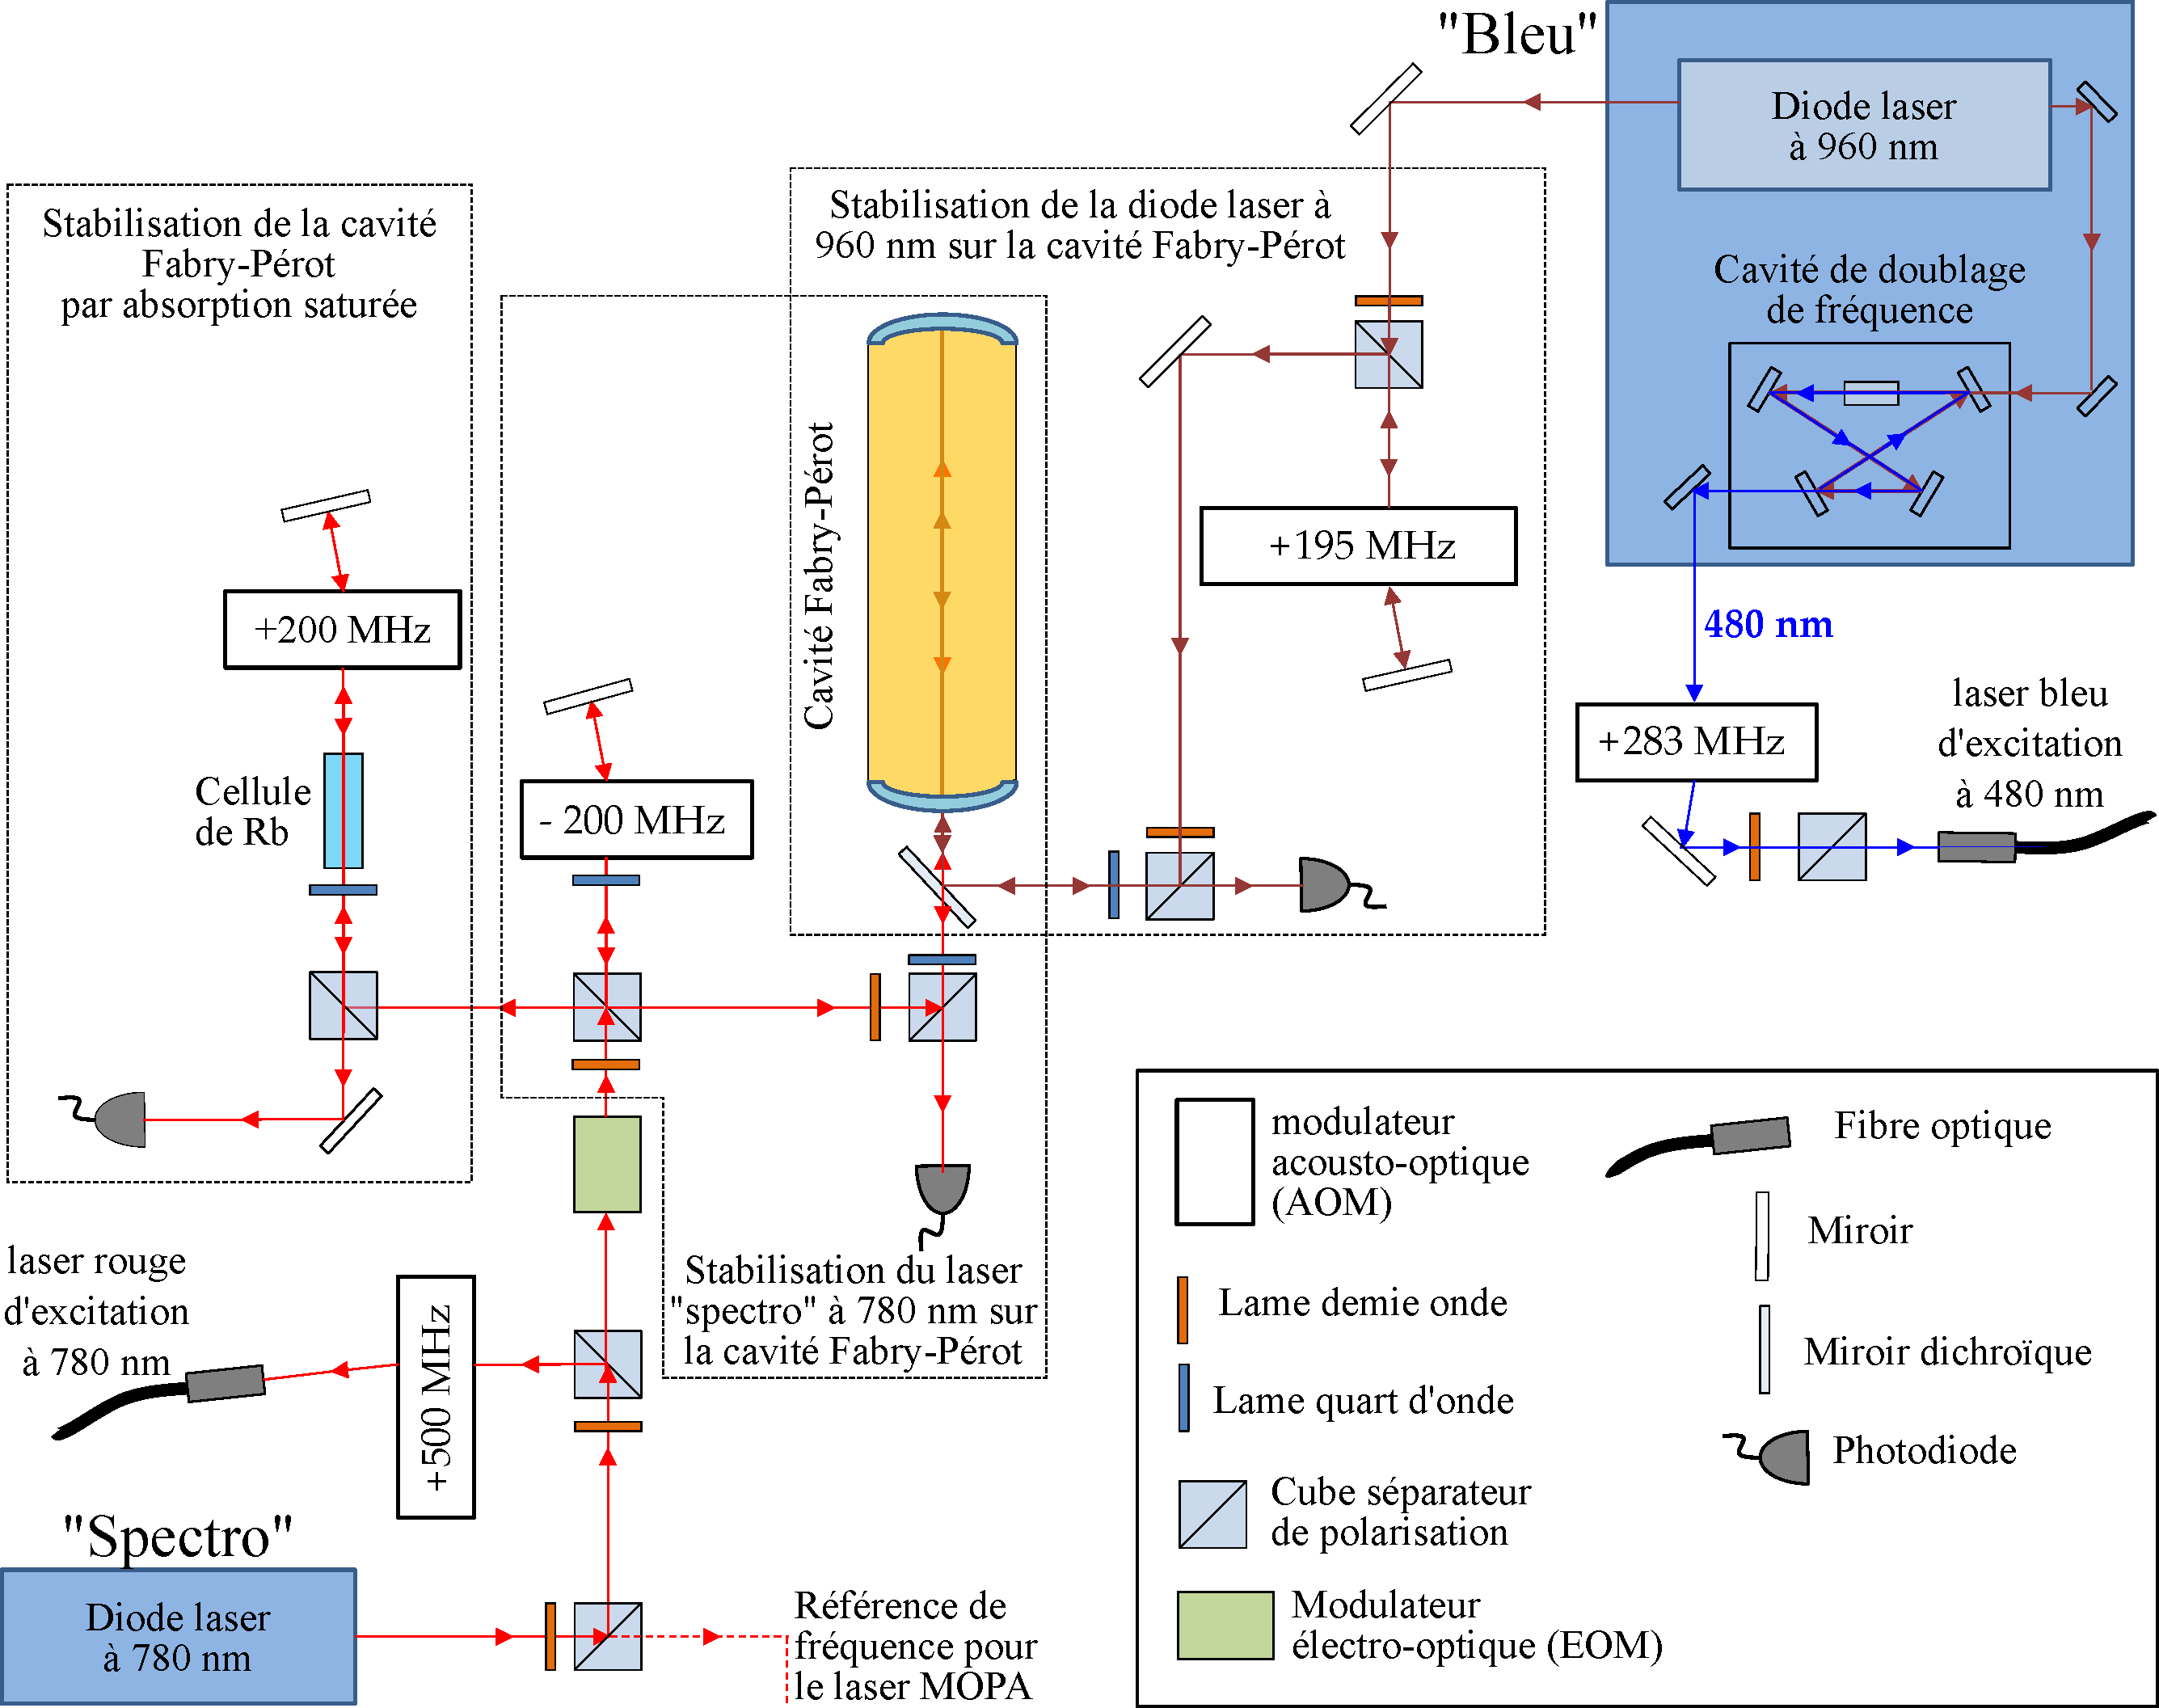
\includegraphics[width=\linewidth]{figures/apx/stabil_laser_1}
\caption[Schéma de stabilisation en fréquence des lasers d'excitation Rydberg]
{
Schéma de stabilisation en fréquence des lasers d'excitation Rydberg.
}
\label{fig:laserlock1}
\end{figure}

\noindent La figure \eqref{fig:laserlock1} présente le schéma de stabilisation en fréquence et de distribution des faisceaux laser qui servent à l'excitation des niveaux de Rydberg.
Le laser \og spectro \fg{} à $\SI{780}{\nano\meter}$ est généré par un système Toptica DL Pro.
Sa fréquence est stabilisée par un circuit Pound-Drever-Hall (PDH), sur un pic de transmission d'une cavité Fabry-Pérot.
La stabilisation PDH nécessite de moduler la phase du faisceau envoyé dans la cavité, ce qui est réalisé grâce à un modulateur électro-optique (EOM), à une fréquence de $\SI{20}{\MHz}$.
La longueur de cette cavité est elle-même stabilisée par absorption saturée, sur le pic intermédiaire (\textit{crossover}) entre les transitions $F=2 \rightarrow F'=2$ et $F=2 \rightarrow F'=3$ du \Rb{87}.

Le laser bleu à $\SI{480}{\nano\meter}$, généré par un système Toptica TA-SHG 110, est obtenu par amplification puis doublage de fréquence de la lumière laser issue d'une diode à $\SI{960}{\nano\meter}$. Le doublage de fréquence est opéré par un cristal non-linéaire de $\mathrm{KNbO_3}$ inséré dans une cavité de doublage \og papillon \fg{}. La fréquence de la diode à $\SI{960}{\nano\meter}$ est stabilisée sur la même cavité Fabry-Pérot que le laser \og spectro \fg{}.
La stabilisation de la diode à $\SI{960}{\nano\meter}$ sur la acvité Fabry-Pérot nécessite de moduler le courant passant dans la diode. Cette modulation est effectuée directement par l'électronique d'alimentation, à une fréquence de $\SI{10}{\MHz}$.
La lumière à $\SI{480}{\nano\meter}$, issue du doublage de la lumière à $\SI{960}{\nano\meter}$ subit ainsi une modulation à une fréquence de $\SI{20}{\MHz}$.

Les deux lasers d'excitation sont finalement déplacés en fréquence par des modulateurs acousto-optiques (AOM) et injectés dans des fibres optiques permettant de les envoyer vers l'expérience.

%\clearpage
La figure \eqref{fig:laserlock2} présente le schéma de stabilisation en fréquence et de distribution des faisceaux laser qui servent au piégeage et au refroidissement du \Rb{87} dans l'état fondamental.
Le laser \og MOPA \fg{} à $\SI{780}{\nano\meter}$ est généré par un système Toptica TA 100.
Sa fréquence est stabilisée par battement (\textit{beatlock}) avec la référence de fréquence donnée par le laser \og spectro \fg{}.
La fréquence du MOPA est décalée de $\SI{-160}{\MHz}$ par rapport à celle du spectro.
La lumière laser issue du MOPA est ensuite divisée afin de fournir les faisceaux de piégeage et de refroidissement pour le piège magnéto-optique 2D, qui fournit le jet atomique vertical permettant d'alimenter l'expérience ;
les faisceaux de piégeage et de refroidissement pour le piège magnéto-optique 3D sur puce ;
le faisceau de pompage optique, permettant de polariser le nuage atomique dans le sous-niveau Zeeman $m_F=+2$ afin de le charger dans le piège magnétique ;
et les deux faisceaux sonde, utilisés pour l'imagerie par absorption.

Tous ces faisceaux sont décalés en fréquence par des AOM puis transportés par fibre optique jusqu'à l'expérience.
Une seule fibre est utilisé pour les faisceaux \og 3D-MOT \fg{} : elle alimente, près de l'expérience, un diviseur de faisceau (\textit{cluster}) qui permet d'obtenir les quatre faisceaux nécessaires au piégeage magnéto-optique des atomes sur la puce.

Enfin, le laser \og repompeur \fg{} à $\SI{780}{\nano\meter}$ est généré par un système Toptica DL Pro.
Sa fréquence est stabilisée par absorption saturée sur la transition $F=1 \rightarrow F'=2$ du \Rb{87}.
Après décalage en fréquence par un AOM, une partie de ce faisceau est transporté par fibre optique à proximité de l'expérience, où il est superposé aux faisceaux du 3D-MOT au sein du \textit{cluster}.
La deuxième partie du faisceau repompeur est superposée aux faisceaux du 2D-MOT avant injection dans leurs fibres optiques respectives.

Tous les coupleurs de fibre optique sont précédés d'obturateurs mécaniques (\textit{shutters}), afin de s'assurer de pouvoir \og éteindre \fg{} complètement chacun des faisceaux qui atteignent l'expérience.
Ces obturateurs ne sont pas représentés sur les figures.

\begin{figure}[h]
\centering
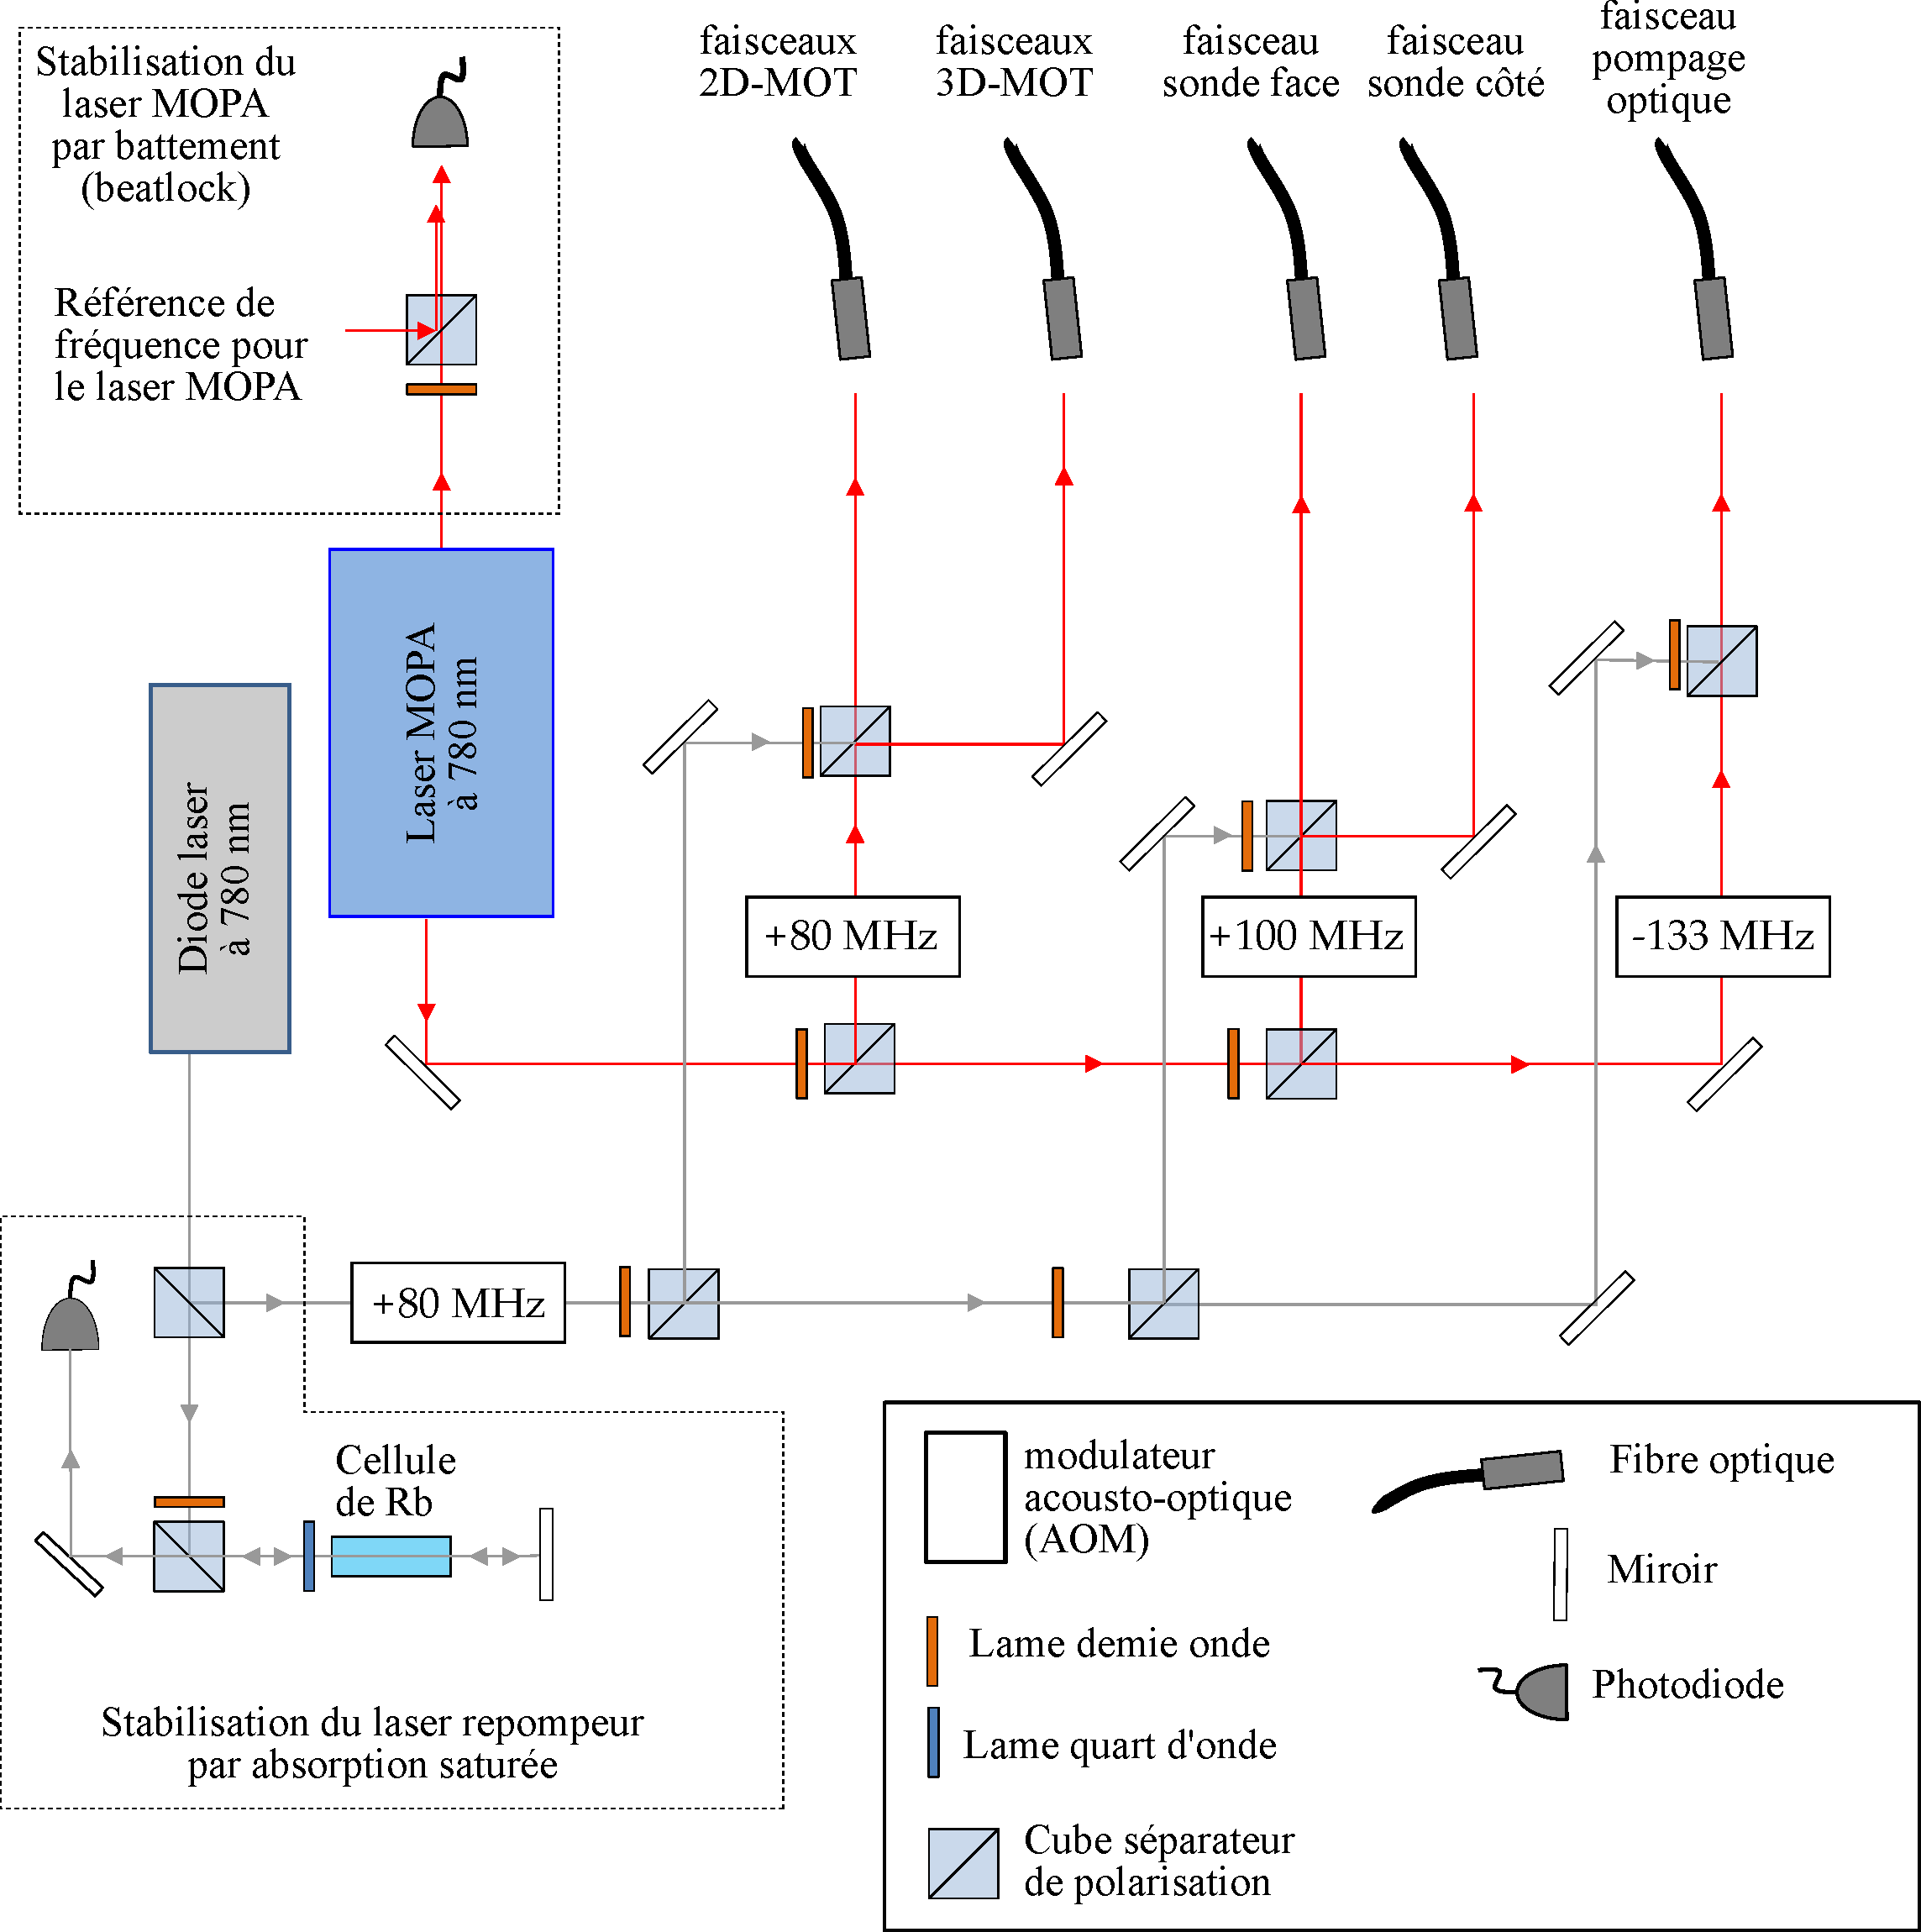
\includegraphics[width=\linewidth]{figures/apx/stabil_laser_2}
\caption[Schéma de stabilisation en fréquence des lasers de piégeage et refroidissement]
{
Schéma de stabilisation en fréquence des lasers de piégeage et refroidissement des atomes dans l'état fondamental.
}
\label{fig:laserlock2}
\end{figure}

\chapter{Détails du fonctionnement de l'algorithme de simulation}\label{app:algo}
\noindent La figure \eqref{fig:algo_sim_spectresoptiques} représente le fonctionnement détaillé de l'algorithme de simulation présenté au chapitre \ref{chapter:60s}.

\begin{figure}[h]
%\centering
\hspace{-.18\linewidth}
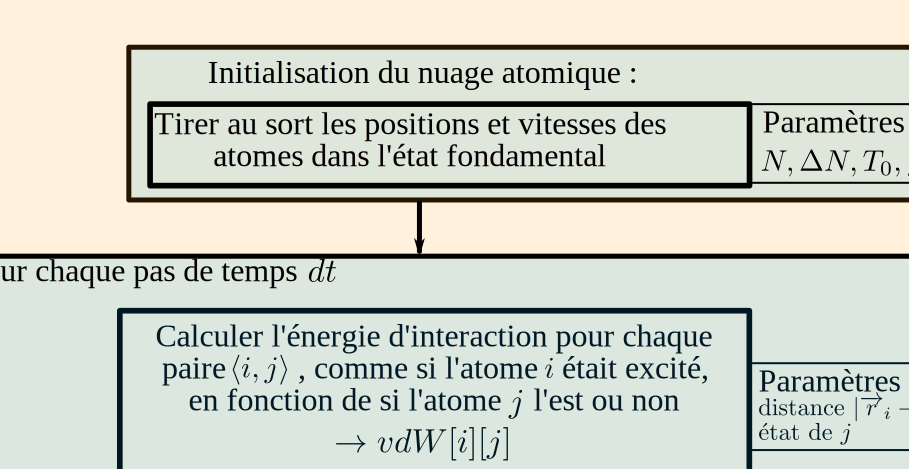
\includegraphics[width=1.3\linewidth]{figures/apx/simus_interactions}
\caption[Schéma fonctionnel de l'algorithme de simulation]
{
Schéma fonctionnel de l'algorithme de simulation.
Cette routine est répétée le nombre d'itérations souhaité, pour différents désaccords laser $\Delta$, afin d'obtenir les spectres simulés.
À chaque fois que le temps $t$ correspond à une durée d'impulsion laser qui nous intéresse, le nombre d'atomes de Rydberg à cet instant est écrit dans un fichier de sortie.
}
\label{fig:algo_sim_spectresoptiques}
\end{figure}
\clearpage